\documentclass[11pt,a4paper]{article}

\usepackage[
    a4paper,
    left=15mm,
    right=15mm,
    top=30mm,
    bottom=25mm,
    headheight=25mm
]{geometry}
\usepackage{graphicx}
\usepackage{polski}
\usepackage[utf8]{inputenc}
\usepackage{enumerate}
\usepackage{comment}
\usepackage{fancyhdr}
\usepackage{hyperref}
\usepackage{indentfirst}
\usepackage{multirow}
\usepackage{multicol}
\usepackage{float}
\usepackage{amsmath}
\usepackage{amssymb}
\usepackage{wrapfig}
\usepackage{layout}
\usepackage{textcomp}
\usepackage[center]{caption}
\usepackage{subcaption}
\usepackage{siunitx}
\usepackage[mathscr]{euscript}
\usepackage{xcolor,colortbl}
\usepackage{setspace}
\usepackage{algorithm}
\usepackage[rightComments=false]{algpseudocodex}
\usepackage{listings}
\usepackage{amsthm}
\usepackage{needspace}

% no lone first/last lines of a paragraph on a page
\widowpenalty=10000
\clubpenalty=10000
\displaywidowpenalty=10000

\sisetup{output-exponent-marker=\ensuremath{\mathrm{e}}, output-decimal-marker={,}}
\algrenewcommand\algorithmicprocedure{\textbf{Procedura}}
\algrenewcommand\algorithmicfor{\textbf{Dla}}
\algrenewcommand\algorithmicdo{\textbf{powtarzaj}}
\algrenewcommand\algorithmicwhile{\textbf{Dopóki}}
\algrenewcommand\algorithmicloop{\textbf{Powtarzaj}}
\algrenewcommand\algorithmicif{\textbf{Jeżeli}}
\algrenewcommand\algorithmicelse{\textbf{Inaczej}}
\algrenewcommand\algorithmicthen{\textbf{wykonaj}}
\algrenewcommand\algorithmicend{\textbf{Koniec}}
\algrenewcommand\algorithmicreturn{\textbf{zwróć}}

\newenvironment{algorytm}[1][htb]
  {\par\bigskip\floatname{algorithm}{}\renewcommand{\thealgorithm}{}
   \begin{algorithm}[#1]%
  }{\end{algorithm}\par\bigskip}

\renewcommand{\baselinestretch}{1.18}
\renewcommand\thesubfigure{\roman{subfigure}}

\renewcommand\lstlistingname{Kod}
\lstset{
    language=Java,
    basicstyle=\ttfamily\footnotesize,
    keywordstyle=\bfseries,
    commentstyle=\itshape\color{gray},
    numbers=left,
    numberstyle=\tiny\color{gray},
    numbersep=8pt,
    frame=tb,
    xleftmargin=6mm,
    columns=fullflexible,
    keepspaces=true,
    showstringspaces=false,
    tabsize=4,
    captionpos=b,
    breaklines=true,
    postbreak=\mbox{\textcolor{gray}{$\hookrightarrow$}\space}
}

\pagestyle{fancy}
\fancyhead[L]{
    
\includegraphics[height=12mm]{img/agh-logo.jpg}
}
\fancyhead[R]{}

\author{Szymon Iwaniuk}
\title{
    
\includegraphics[height=45mm]{img/agh-logo.jpg}
    \vspace{10mm}
    \\
    Problem pięciu filozofów}
\date{Teoria Współbieżności 2025/2026, laboratorium 5 \\ 8 listopada 2026}

\begin{document}

\maketitle
\tableofcontents
\pagebreak

\section{Wstęp}
\subsection{Treść zadania}
Celem ćwiczenia jest zapoznanie się z jednym z klasycznych problemów teorii współbieżności --
problemem pięciu filozofów (autor E.W. Dijkstra).

\begin{figure}[H]
    \centering
    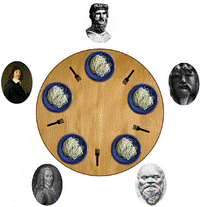
\includegraphics[width=55mm]{img/filozofowie.png}
    \caption{Problem pięciu filozofów}
\end{figure}

\begin{itemize}
    \item Każdy filozof zajmuje się głównie myśleniem.
    \item Od czasu do czasu potrzebuje zjeść.
    \item Do jedzenia potrzebne mu są oba widelce po jego prawej i lewej stronie.
    \item Jedzenie trwa skończoną (ale nieokreśloną z góry) ilość czasu, po czym filozof widelce
          odkłada i wraca do myślenia.
    \item Cykl powtarza się od początku.
\end{itemize}

Ćwiczenia (na podstawie szkieletu programu \texttt{Fil5mon.java}):
\begin{enumerate}[a)]
    \item Zaimplementować trywialne rozwiązanie z symetrycznymi filozofami. Zaobserwować problem blokady.
    \item Zaimplementować rozwiązanie z widelcami podnoszonymi jednocześnie. Jaki problem może tutaj wystąpić?
    \item Zaimplementować rozwiązanie z lokajem.
    \item Wykonać pomiary dla każdego rozwiązania i wywnioskować, co ma wpływ na wydajność każdego rozwiązania.
\end{enumerate}
Dodatkowe zadanie: zaproponować autorskie rozwiązanie, inne niż powyższe.

\subsection{Opis rozwiązania}
Porównujemy cztery implementacje stołu, wszystkie oparte na monitorach Javy
(\texttt{synchronized}, \texttt{wait()}, \texttt{notify()}):
\begin{itemize}
    \item \textbf{a) trywialne} -- każdy filozof podnosi najpierw lewy, potem prawy widelec,
    \item \textbf{b) oba widelce naraz} -- jeden monitor stołu, filozof czeka, aż oba jego widelce
          będą wolne, i zabiera je w jednym kroku,
    \item \textbf{c) lokaj} -- jak a), ale do stołu jednocześnie dopuszczonych jest co najwyżej $n - 1$ filozofów,
    \item \textbf{asymetryczne (autorskie)} -- każdy filozof podnosi najpierw widelec o mniejszym numerze,
          więc ostatni filozof podnosi widelce w odwrotnej kolejności niż pozostali.
\end{itemize}
Program działa dla dowolnej liczby filozofów $n$, a nie tylko dla pięciu, dzięki czemu można zbadać,
jak rozwiązania skalują się z wielkością stołu.

Razem ze sprawozdaniem zawarty jest kod w języku \texttt{Java} zawierający wszystkie implementacje,
program wykonujący pomiary oraz skrypt służący do generowania zawartych w dokumencie wykresów.

\section{Specyfikacja narzędzi i sprzętu}
Program został napisany w języku \texttt{Java 27} i uruchomiony na maszynie wirtualnej
\texttt{OpenJDK}, na komputerze z procesorem \texttt{Apple M4} (architektura \texttt{ARM64},
10 rdzeni: 4 wydajnościowe i 6 energooszczędnych), \texttt{16 GB} zunifikowanej pamięci
\texttt{LPDDR5} i systemem operacyjnym \texttt{macOS 26}.
Do wygenerowania wykresów użyty został \texttt{Python} z biblioteką \texttt{matplotlib}.

\subsection{Metoda pomiaru}
Filozof w pętli myśli, staje się głodny, zdobywa oba widelce, je i odkłada widelce.
Czasy myślenia i jedzenia są losowane z rozkładu jednostajnego na przedziale $[0, 2t)$,
gdzie $t$ to średni czas danego scenariusza. Opóźnienie realizujemy przez \texttt{LockSupport.parkNanos},
więc wątek nie zajmuje procesora. Badamy cztery scenariusze (średni czas myślenia / jedzenia):
\begin{itemize}
    \item \textbf{0/0} -- bez myślenia i jedzenia, mierzymy wyłącznie koszt synchronizacji,
    \item \textbf{0/1} -- myślenie 0 ms, jedzenie 1 ms, filozofowie są cały czas głodni (największa rywalizacja),
    \item \textbf{1/1} -- myślenie 1 ms, jedzenie 1 ms,
    \item \textbf{10/1} -- myślenie 10 ms, jedzenie 1 ms (mała rywalizacja).
\end{itemize}

Każdy przebieg trwa 1 s, a wszystkie wątki startują jednocześnie po zwolnieniu zatrzasku
\texttt{CountDownLatch}. Każdy filozof liczy swoje posiłki oraz czas oczekiwania na widelce,
czyli czas od zgłoszenia głodu do rozpoczęcia jedzenia (\texttt{System.nanoTime()}).
Na tej podstawie wyznaczamy przepustowość (liczba posiłków na sekundę),
średni i maksymalny czas oczekiwania oraz indeks Jaina liczby posiłków
\[
    J(x_1, \dots, x_n) = \frac{\left(\sum_{i=1}^{n} x_i\right)^2}{n \sum_{i=1}^{n} x_i^2},
\]
gdzie $x_i$ to liczba posiłków $i$-tego filozofa. $J = 1$, gdy wszyscy zjedli tyle samo razy,
a $J = \frac{1}{n}$, gdy jadł tylko jeden filozof. Przed pomiarami wykonujemy kilka przebiegów
rozgrzewających kompilator JIT, a każdą konfigurację uruchamiamy trzy razy i bierzemy medianę.
Parametry: $n \in \{5, 10, 20, 50, 100\}$.

Rozwiązanie trywialne badamy osobno: przebieg kończy się w chwili wykrycia blokady
(albo po 1 s), a każdą konfigurację $n \in \{5, 10, 20, 50\}$ uruchamiamy 20 razy.
Blokadę wykrywamy dokładnie: stół liczy filozofów, którzy trzymają lewy widelec i czekają
na prawy. Gdy jest ich $n$, wszystkie widelce są zajęte i żaden filozof nie może kontynuować.

Ostatni eksperyment sprawdza zagłodzenie: przy $n = 5$ filozofowie F1 i F3 (,,żarłoki'')
w ogóle nie myślą i jedzą średnio 2 ms, a pozostali myślą 10 ms i jedzą 1 ms. Przebieg trwa 3 s.

W każdym przebiegu filozof po zdobyciu widelców sprawdza, czy żaden z jego sąsiadów nie je.
Takie zdarzenie przerwałoby pomiary wyjątkiem -- we wszystkich przebiegach nie wystąpiło.

\section{Algorytmy}
Filozof $i$ korzysta z widelca $i$ (lewego) i widelca $(i + 1) \bmod n$ (prawego).
Wszystkie rozwiązania różnią się tylko procedurami \textsc{acquire} i \textsc{release},
pętla filozofa jest wspólna.

\begin{algorytm}[H]
\setstretch{1.4}
\begin{algorithmic}[1]
    \Procedure{filozof}{$i$}
        \Loop
            \State myśl
            \State $t_0 \gets$ \textsc{now}()
            \State \Call{acquire}{$i$}
            \State zapisz czas oczekiwania \textsc{now}() $- t_0$
            \State jedz
            \State \Call{release}{$i$}
        \EndLoop
    \EndProcedure
\end{algorithmic}
\caption{Pętla filozofa}
\end{algorytm}

Widelec w rozwiązaniach a), c) i asymetrycznym jest monitorem działającym jak semafor binarny.

\begin{algorytm}[H]
\setstretch{1.4}
\begin{algorithmic}[1]
    \Procedure{take}{$w$} \Comment{\texttt{synchronized}}
        \While{$w.\textit{zajęty}$}
            \State \textsc{wait}()
        \EndWhile
        \State $w.\textit{zajęty} \gets \texttt{true}$
    \EndProcedure
    \Procedure{put}{$w$} \Comment{\texttt{synchronized}}
        \State $w.\textit{zajęty} \gets \texttt{false}$, \ \textsc{notify}()
    \EndProcedure
\end{algorithmic}
\caption{Widelec}
\end{algorytm}

\needspace{14\baselineskip}
\subsection{Rozwiązanie trywialne}
\begin{algorytm}[H]
\setstretch{1.4}
\begin{algorithmic}[1]
    \Procedure{acquire}{$i$}
        \State \Call{take}{$\textit{widelec}[i]$}
        \State \Call{take}{$\textit{widelec}[(i + 1) \bmod n]$}
    \EndProcedure
    \Procedure{release}{$i$}
        \State \Call{put}{$\textit{widelec}[(i + 1) \bmod n]$}, \ \Call{put}{$\textit{widelec}[i]$}
    \EndProcedure
\end{algorithmic}
\caption{Rozwiązanie trywialne}
\end{algorytm}

Jeżeli wszyscy filozofowie jednocześnie wykonają wiersz 2, każdy trzyma swój lewy widelec,
a jego prawy widelec jest lewym widelcem sąsiada. Spełnione są wszystkie cztery warunki
Coffmana: wzajemne wykluczanie, trzymanie zasobu podczas oczekiwania, brak wywłaszczania
oraz cykl oczekiwania $F_0 \to F_1 \to \dots \to F_{n-1} \to F_0$. Dochodzi do blokady (zakleszczenia).

\needspace{16\baselineskip}
\subsection{Rozwiązanie z widelcami podnoszonymi jednocześnie}
\begin{algorytm}[H]
\setstretch{1.4}
\begin{algorithmic}[1]
    \Procedure{acquire}{$i$} \Comment{\texttt{synchronized} na całym stole}
        \While{$\textit{zajęty}[i] \lor \textit{zajęty}[(i + 1) \bmod n]$}
            \State \textsc{wait}()
        \EndWhile
        \State $\textit{zajęty}[i] \gets \texttt{true}$, \ $\textit{zajęty}[(i + 1) \bmod n] \gets \texttt{true}$
    \EndProcedure
    \Procedure{release}{$i$} \Comment{\texttt{synchronized} na całym stole}
        \State $\textit{zajęty}[i] \gets \texttt{false}$, \ $\textit{zajęty}[(i + 1) \bmod n] \gets \texttt{false}$
        \State \textsc{notifyAll}() \Comment{obaj sąsiedzi mogą czekać}
    \EndProcedure
\end{algorithmic}
\caption{Widelce podnoszone jednocześnie}
\end{algorytm}

Filozof nigdy nie trzyma jednego widelca, czekając na drugi, więc warunek ,,trzymaj i czekaj''
nie jest spełniony i blokada jest niemożliwa. Pojawia się za to \textbf{zagłodzenie}: filozof $i$
może jeść tylko wtedy, gdy jednocześnie nie je żaden z jego sąsiadów. Jeżeli sąsiedzi jedzą
na zmianę tak, że zawsze je co najmniej jeden z nich, filozof $i$ czeka w nieskończoność,
mimo że cały system działa. Dodatkowo cały stół jest jednym monitorem, a \textsc{notifyAll}
budzi wszystkich czekających, chociaż jeść mogą co najwyżej dwaj sąsiedzi zwalniającego.

\needspace{18\baselineskip}
\subsection{Rozwiązanie z lokajem}
\begin{algorytm}[H]
\setstretch{1.4}
\begin{algorithmic}[1]
    \Procedure{acquire}{$i$}
        \State \textbf{synchronized}(\textit{lokaj}): \textbf{dopóki} $\textit{przy stole} = n - 1$ \textsc{wait}(); \ $\textit{przy stole} \gets \textit{przy stole} + 1$
        \State \Call{take}{$\textit{widelec}[i]$}
        \State \Call{take}{$\textit{widelec}[(i + 1) \bmod n]$}
    \EndProcedure
    \Procedure{release}{$i$}
        \State \Call{put}{$\textit{widelec}[(i + 1) \bmod n]$}, \ \Call{put}{$\textit{widelec}[i]$}
        \State \textbf{synchronized}(\textit{lokaj}): $\textit{przy stole} \gets \textit{przy stole} - 1$, \ \textsc{notify}()
    \EndProcedure
\end{algorithmic}
\caption{Rozwiązanie z lokajem}
\end{algorytm}

Przy stole jest co najwyżej $n - 1$ filozofów, a widelców jest $n$. Z zasady szufladkowej
co najmniej jeden filozof przy stole ma dostęp do obu swoich widelców, więc cykl oczekiwania
nie może się zamknąć. Lokaj jest jednak wspólnym monitorem, przez który przechodzi każdy posiłek.

\needspace{14\baselineskip}
\subsection{Rozwiązanie asymetryczne (autorskie)}
\begin{algorytm}[H]
\setstretch{1.4}
\begin{algorithmic}[1]
    \Procedure{acquire}{$i$}
        \State $a \gets \min(i, (i + 1) \bmod n)$, \ $b \gets \max(i, (i + 1) \bmod n)$
        \State \Call{take}{$\textit{widelec}[a]$}, \ \Call{take}{$\textit{widelec}[b]$}
    \EndProcedure
    \Procedure{release}{$i$}
        \State \Call{put}{$\textit{widelec}[b]$}, \ \Call{put}{$\textit{widelec}[a]$}
    \EndProcedure
\end{algorithmic}
\caption{Rozwiązanie asymetryczne (hierarchia zasobów)}
\end{algorytm}

Widelce są ponumerowane, a każdy filozof podnosi je w kolejności rosnących numerów.
Dla filozofów $0, \dots, n-2$ oznacza to lewy, potem prawy widelec, a filozof $n - 1$
(widelce $n - 1$ i $0$) podnosi najpierw prawy. W cyklu oczekiwania każdy wątek czekałby
na widelec o większym numerze niż ten, który trzyma, co jest niemożliwe w zamkniętym cyklu.
Rozwiązanie nie wymaga żadnego wspólnego monitora -- każdy widelec synchronizuje tylko
dwóch sąsiadów.

\pagebreak
\section{Implementacja}
Poniżej znajduje się pełny kod programu. Każda klasa jest w osobnym pliku w katalogu \texttt{src}.

Klasa \textbf{Fork} to widelec ze szkieletu programu (\texttt{Widelec}) zrealizowany jako monitor.

\begin{lstlisting}[caption={Klasa \textbf{Fork} (\texttt{src/Fork.java})}]
/** Fork as a Java monitor, like Widelec from the skeleton: take() waits until the fork is free. */
class Fork {
    private boolean taken = false;

    synchronized void take() throws InterruptedException {
        while (taken) wait();
        taken = true;
    }

    synchronized void put() {
        taken = false;
        notify();
    }
}
\end{lstlisting}

Klasa \textbf{Table} jest wspólną bazą wszystkich rozwiązań. Metoda \texttt{create} wybiera implementację po nazwie.

\begin{lstlisting}[caption={Klasa \textbf{Table} (\texttt{src/Table.java})}]
/**
 * Common base of all solutions. Philosopher i uses fork i (left) and fork (i+1) mod n (right);
 * acquire(i) returns when philosopher i holds both forks, release(i) puts them back.
 */
abstract class Table {
    final int n;

    Table(int n) {
        this.n = n;
    }

    int left(int i) {
        return i;
    }

    int right(int i) {
        return (i + 1) % n;
    }

    abstract void acquire(int i) throws InterruptedException;

    abstract void release(int i);

    /** True when the table is certainly in a deadlock (only the naive solution can be). */
    boolean deadlocked() {
        return false;
    }

    static Fork[] forks(int n) {
        Fork[] forks = new Fork[n];
        for (int i = 0; i < n; i++) forks[i] = new Fork();
        return forks;
    }

    static Table create(String impl, int n) {
        return switch (impl) {
            case "naive" -> new NaiveTable(n);
            case "both" -> new BothTable(n);
            case "waiter" -> new WaiterTable(n);
            case "asym" -> new AsymmetricTable(n);
            default -> throw new IllegalArgumentException(impl);
        };
    }
}
\end{lstlisting}

Klasa \textbf{NaiveTable} to rozwiązanie trywialne a). Licznik \texttt{holdingOne} służy wyłącznie do wykrywania blokady.

\begin{lstlisting}[caption={Klasa \textbf{NaiveTable} (\texttt{src/NaiveTable.java})}]
import java.util.concurrent.atomic.AtomicInteger;

/** a) Symmetric philosophers: left fork first, then right fork. Can deadlock. */
class NaiveTable extends Table {
    private final Fork[] forks;
    // philosophers holding their left fork and not yet the right one
    private final AtomicInteger holdingOne = new AtomicInteger();

    NaiveTable(int n) {
        super(n);
        forks = forks(n);
    }

    @Override
    void acquire(int i) throws InterruptedException {
        forks[left(i)].take();
        holdingOne.incrementAndGet();
        forks[right(i)].take();
        holdingOne.decrementAndGet();
    }

    @Override
    void release(int i) {
        forks[right(i)].put();
        forks[left(i)].put();
    }

    /** All n philosophers hold one fork each and wait for the other: nobody can ever continue. */
    @Override
    boolean deadlocked() {
        return holdingOne.get() == n;
    }
}
\end{lstlisting}

Klasa \textbf{BothTable} to rozwiązanie b) z widelcami podnoszonymi jednocześnie.

\begin{lstlisting}[caption={Klasa \textbf{BothTable} (\texttt{src/BothTable.java})}]
/**
 * b) Both forks taken at once: one monitor for the whole table, a philosopher waits
 * until both forks are free and takes them in one step. No deadlock, but
 * a philosopher whose neighbours eat in turns can starve.
 */
class BothTable extends Table {
    private final boolean[] taken;

    BothTable(int n) {
        super(n);
        taken = new boolean[n];
    }

    @Override
    synchronized void acquire(int i) throws InterruptedException {
        while (taken[left(i)] || taken[right(i)]) wait();
        taken[left(i)] = true;
        taken[right(i)] = true;
    }

    @Override
    synchronized void release(int i) {
        taken[left(i)] = false;
        taken[right(i)] = false;
        notifyAll(); // both neighbours may be waiting
    }
}
\end{lstlisting}

Klasy \textbf{Waiter} i \textbf{WaiterTable} to rozwiązanie c) z lokajem.

\begin{lstlisting}[caption={Klasa \textbf{Waiter} (\texttt{src/Waiter.java})}]
/** Waiter (lokaj) lets at most limit philosophers try to take forks at the same time. */
class Waiter {
    private final int limit;
    private int seated = 0;

    Waiter(int limit) {
        this.limit = limit;
    }

    synchronized void enter() throws InterruptedException {
        while (seated == limit) wait();
        seated++;
    }

    synchronized void leave() {
        seated--;
        notify(); // exactly one place became free
    }
}
\end{lstlisting}

\begin{lstlisting}[caption={Klasa \textbf{WaiterTable} (\texttt{src/WaiterTable.java})}]
/** c) Naive fork order guarded by a waiter that admits at most n - 1 philosophers. */
class WaiterTable extends Table {
    private final Fork[] forks;
    private final Waiter waiter;

    WaiterTable(int n) {
        super(n);
        forks = forks(n);
        waiter = new Waiter(n - 1);
    }

    @Override
    void acquire(int i) throws InterruptedException {
        waiter.enter();
        forks[left(i)].take();
        forks[right(i)].take();
    }

    @Override
    void release(int i) {
        forks[right(i)].put();
        forks[left(i)].put();
        waiter.leave();
    }
}
\end{lstlisting}

Klasa \textbf{AsymmetricTable} to rozwiązanie autorskie z hierarchią widelców.

\begin{lstlisting}[caption={Klasa \textbf{AsymmetricTable} (\texttt{src/AsymmetricTable.java})}]
/**
 * Own solution: resource ordering. Every philosopher takes the fork with the lower number
 * first, so the last one (forks n-1 and 0) takes the right fork first. No central monitor.
 */
class AsymmetricTable extends Table {
    private final Fork[] forks;

    AsymmetricTable(int n) {
        super(n);
        forks = forks(n);
    }

    @Override
    void acquire(int i) throws InterruptedException {
        forks[Math.min(left(i), right(i))].take();
        forks[Math.max(left(i), right(i))].take();
    }

    @Override
    void release(int i) {
        forks[Math.max(left(i), right(i))].put();
        forks[Math.min(left(i), right(i))].put();
    }
}
\end{lstlisting}

Klasa \textbf{Philosopher} to wątek filozofa ze szkieletu (\texttt{Filozof}) rozszerzony o pomiary i sprawdzenie, czy sąsiedzi nie jedzą jednocześnie.

\begin{lstlisting}[caption={Klasa \textbf{Philosopher} (\texttt{src/Philosopher.java})}]
import java.util.SplittableRandom;
import java.util.concurrent.CountDownLatch;
import java.util.concurrent.atomic.AtomicIntegerArray;
import java.util.concurrent.locks.LockSupport;

/**
 * Thinks and eats for random times (uniform on [0, 2 * mean)) until stop is set,
 * recording the number of meals and the time spent waiting for forks.
 */
class Philosopher extends Thread {
    private final int id;
    private final Table table;
    private final long thinkNs, eatNs;
    private final SplittableRandom rnd;
    private final AtomicIntegerArray eating; // shared, used to check mutual exclusion
    private final CountDownLatch start;
    private volatile boolean stop = false;
    long meals = 0, waitSumNs = 0, waitMaxNs = 0;

    Philosopher(int id, Table table, long thinkNs, long eatNs, long seed,
                AtomicIntegerArray eating, CountDownLatch start) {
        this.id = id;
        this.table = table;
        this.thinkNs = thinkNs;
        this.eatNs = eatNs;
        this.rnd = new SplittableRandom(seed);
        this.eating = eating;
        this.start = start;
    }

    void finish() {
        stop = true;
    }

    private void pause(long meanNs) {
        if (meanNs == 0) return;
        long end = System.nanoTime() + rnd.nextLong(2 * meanNs);
        long left;
        while ((left = end - System.nanoTime()) > 0) LockSupport.parkNanos(left);
    }

    @Override
    public void run() {
        int n = table.n;
        try {
            start.await();
            while (!stop) {
                pause(thinkNs);                                   // thinking
                long t0 = System.nanoTime();
                table.acquire(id);                                // hungry
                long wait = System.nanoTime() - t0;
                eating.set(id, 1);
                if (eating.get((id + 1) % n) == 1 || eating.get((id + n - 1) % n) == 1)
                    throw new IllegalStateException("neighbours of " + id + " eat at the same time");
                meals++;
                waitSumNs += wait;
                waitMaxNs = Math.max(waitMaxNs, wait);
                pause(eatNs);                                     // eating
                eating.set(id, 0);
                table.release(id);
            }
        } catch (InterruptedException e) {
            // stopped while waiting, only happens after a deadlock
        }
    }
}
\end{lstlisting}

Klasa \textbf{Main} wykonuje wszystkie trzy eksperymenty i zapisuje wyniki do plików CSV, z których skrypt w Pythonie rysuje wykresy.

\begin{lstlisting}[caption={Klasa \textbf{Main} (\texttt{src/Main.java})}]
import java.io.FileWriter;
import java.io.IOException;
import java.io.PrintWriter;
import java.util.Arrays;
import java.util.concurrent.CountDownLatch;
import java.util.concurrent.atomic.AtomicIntegerArray;
import java.util.concurrent.atomic.AtomicReference;
import java.util.concurrent.locks.LockSupport;

/**
 * Three experiments, results in csv/:
 * runs.csv       - deadlock-free solutions, throughput, waiting time and fairness vs n and scenario,
 * deadlock.csv   - naive solution, time until deadlock,
 * starvation.csv - n = 5 with two greedy philosophers, meals of every philosopher.
 */
public class Main {
    static final String[] IMPLS = {"both", "waiter", "asym"};
    static final int[] SIZES = {5, 10, 20, 50, 100};
    static final int[] DEADLOCK_SIZES = {5, 10, 20, 50};
    static final long MS = 1_000_000L;
    /** name, mean thinking time, mean eating time [ns] */
    record Scenario(String name, long thinkNs, long eatNs) {}
    static final Scenario[] SCENARIOS = {
            new Scenario("0/0", 0, 0),
            new Scenario("0/1", 0, MS),
            new Scenario("1/1", MS, MS),
            new Scenario("10/1", 10 * MS, MS),
    };
    static final long RUN_NS = 1000 * MS;
    static final int REPS = 3;
    static final int DEADLOCK_REPS = 20;
    static final long STARVE_NS = 3000 * MS;

    record Result(long timeNs, boolean deadlock, long[] meals, double[] perMeanUs, double[] perMaxUs) {
        long totalMeals() {
            return Arrays.stream(meals).sum();
        }

        double meanWaitUs() {
            double sum = 0;
            for (int i = 0; i < meals.length; i++) sum += perMeanUs[i] * meals[i];
            return totalMeals() == 0 ? 0 : sum / totalMeals();
        }

        double maxWaitUs() {
            return Arrays.stream(perMaxUs).max().orElse(0);
        }

        /** Jain's index of meals: 1 when everybody ate the same number of times, 1/n when one ate. */
        double jain() {
            double sum = 0, sumSq = 0;
            for (long m : meals) {
                sum += m;
                sumSq += (double) m * m;
            }
            return sumSq == 0 ? 0 : sum * sum / (meals.length * sumSq);
        }
    }

    static Result run(String impl, long[] think, long[] eat, long limitNs, long seed) throws InterruptedException {
        int n = think.length;
        Table table = Table.create(impl, n);
        AtomicIntegerArray eating = new AtomicIntegerArray(n);
        AtomicReference<Throwable> error = new AtomicReference<>();
        CountDownLatch start = new CountDownLatch(1);
        Philosopher[] ph = new Philosopher[n];
        for (int i = 0; i < n; i++) {
            ph[i] = new Philosopher(i, table, think[i], eat[i], seed * 1_000 + i, eating, start);
            ph[i].setUncaughtExceptionHandler((t, e) -> error.compareAndSet(null, e));
            ph[i].start();
        }
        long t0 = System.nanoTime();
        start.countDown();
        boolean deadlock = false;
        while (System.nanoTime() - t0 < limitNs) {
            if (table.deadlocked()) {
                deadlock = true;
                break;
            }
            LockSupport.parkNanos(100_000);
        }
        long elapsed = System.nanoTime() - t0;
        for (Philosopher p : ph) p.finish();
        if (deadlock) for (Philosopher p : ph) p.interrupt();
        for (Philosopher p : ph) p.join();
        if (error.get() != null) throw new IllegalStateException(impl, error.get());

        long[] meals = new long[n];
        double[] mean = new double[n], max = new double[n];
        for (int i = 0; i < n; i++) {
            meals[i] = ph[i].meals;
            mean[i] = meals[i] == 0 ? 0 : ph[i].waitSumNs / 1e3 / meals[i];
            max[i] = ph[i].waitMaxNs / 1e3;
        }
        return new Result(elapsed, deadlock, meals, mean, max);
    }

    static long[] same(int n, long v) {
        long[] a = new long[n];
        Arrays.fill(a, v);
        return a;
    }

    public static void main(String[] args) throws IOException, InterruptedException {
        String out = args.length > 0 ? args[0] : "csv";

        // JIT warm-up, results discarded
        for (String impl : IMPLS)
            for (int i = 0; i < 3; i++) run(impl, same(10, 0), same(10, 0), 300 * MS, i);

        try (PrintWriter w = new PrintWriter(new FileWriter(out + "/runs.csv"))) {
            w.println("impl,scenario,n,rep,time_ms,meals,throughput,mean_wait_us,max_wait_us,jain");
            for (Scenario s : SCENARIOS)
                for (int n : SIZES)
                    for (String impl : IMPLS)
                        for (int r = 0; r < REPS; r++) {
                            Result res = run(impl, same(n, s.thinkNs()), same(n, s.eatNs()), RUN_NS, r);
                            if (res.deadlock()) throw new IllegalStateException(impl + " deadlocked");
                            double sec = res.timeNs() / 1e9;
                            w.printf("%s,%s,%d,%d,%.3f,%d,%.1f,%.3f,%.3f,%.4f%n", impl, s.name(), n, r,
                                    res.timeNs() / 1e6, res.totalMeals(), res.totalMeals() / sec,
                                    res.meanWaitUs(), res.maxWaitUs(), res.jain());
                            System.out.printf("%-5s n=%-3d %-6s rep %d: %10.0f meals/s, wait %9.1f us, J=%.3f%n",
                                    s.name(), n, impl, r, res.totalMeals() / sec, res.meanWaitUs(), res.jain());
                        }
        }

        try (PrintWriter w = new PrintWriter(new FileWriter(out + "/deadlock.csv"))) {
            w.println("scenario,n,rep,deadlock,time_ms,meals");
            for (Scenario s : SCENARIOS)
                for (int n : DEADLOCK_SIZES)
                    for (int r = 0; r < DEADLOCK_REPS; r++) {
                        Result res = run("naive", same(n, s.thinkNs()), same(n, s.eatNs()), RUN_NS, r);
                        w.printf("%s,%d,%d,%d,%.3f,%d%n", s.name(), n, r, res.deadlock() ? 1 : 0,
                                res.timeNs() / 1e6, res.totalMeals());
                        System.out.printf("%-5s n=%-3d naive  rep %2d: %s after %8.2f ms, %d meals%n", s.name(), n, r,
                                res.deadlock() ? "DEADLOCK" : "no deadlock", res.timeNs() / 1e6, res.totalMeals());
                    }
        }

        // philosophers 1 and 3 never think and eat 2 ms, the others think 10 ms and eat 1 ms
        long[] think = {10 * MS, 0, 10 * MS, 0, 10 * MS};
        long[] eat = {MS, 2 * MS, MS, 2 * MS, MS};
        try (PrintWriter w = new PrintWriter(new FileWriter(out + "/starvation.csv"))) {
            w.println("impl,rep,philosopher,meals,mean_wait_us,max_wait_us");
            for (String impl : IMPLS)
                for (int r = 0; r < REPS; r++) {
                    Result res = run(impl, think, eat, STARVE_NS, r);
                    for (int i = 0; i < 5; i++)
                        w.printf("%s,%d,%d,%d,%.3f,%.3f%n", impl, r, i, res.meals()[i], res.perMeanUs()[i], res.perMaxUs()[i]);
                    System.out.printf("starvation %-6s rep %d: meals %s%n", impl, r, Arrays.toString(res.meals()));
                }
        }
    }
}
\end{lstlisting}

\pagebreak
\section{Wyniki}
\subsection{Blokada w rozwiązaniu trywialnym}
\textbf{Rysunek 2} pokazuje czas do wystąpienia blokady oraz odsetek przebiegów,
w których blokada wystąpiła w ciągu 1 s.

\begin{figure}[H]
    \centering
    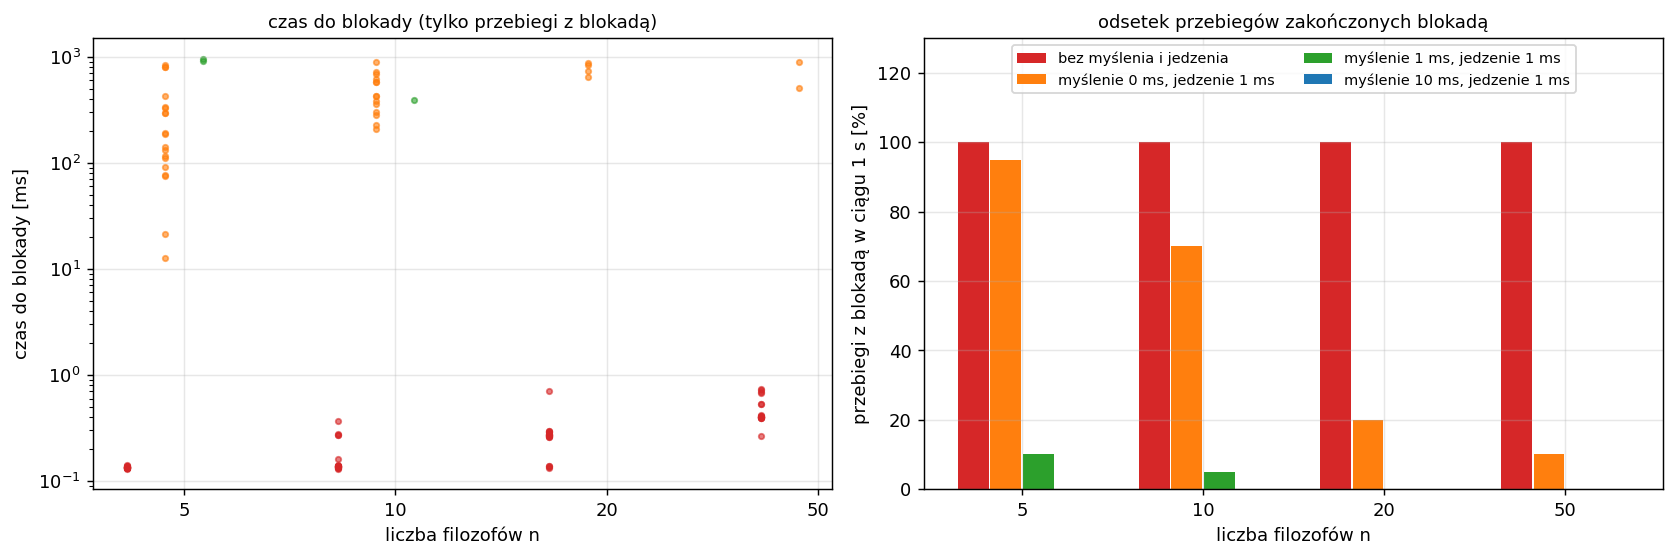
\includegraphics[width=\textwidth]{img/deadlock.png}
    \caption{Blokada w rozwiązaniu trywialnym (20 przebiegów na konfigurację)}
\end{figure}

Bez myślenia i jedzenia blokada wystąpiła w każdym przebiegu, a mediana czasu do blokady
wynosi 0,14 ms dla $n = 5$ i 0,41 ms dla $n = 50$ (filozofowie zdążyli zjeść łącznie
odpowiednio 98 i 1577 razy). Przy ciągle głodnych filozofach i jedzeniu 1 ms blokada wystąpiła
w 95\% przebiegów dla $n = 5$ (mediana 186 ms), ale tylko w 20\% dla $n = 20$ i 10\% dla $n = 50$.
Gdy filozofowie myślą 1 ms, blokada w ciągu sekundy zdarzała się rzadko (10\% dla $n = 5$),
a przy 10 ms myślenia nie wystąpiła ani razu.

Blokada wymaga, żeby wszyscy filozofowie jednocześnie trzymali lewy widelec.
Im krótsze myślenie i im mniej filozofów, tym większe szanse na takie ułożenie,
dlatego rozwiązanie trywialne wydaje się działać poprawnie przy małej rywalizacji.
Nie jest jednak poprawne -- blokada jest tylko kwestią czasu.

\subsection{Przepustowość}
\textbf{Rysunek 3} pokazuje liczbę posiłków na sekundę dla rozwiązań wolnych od blokady.

\begin{figure}[H]
    \centering
    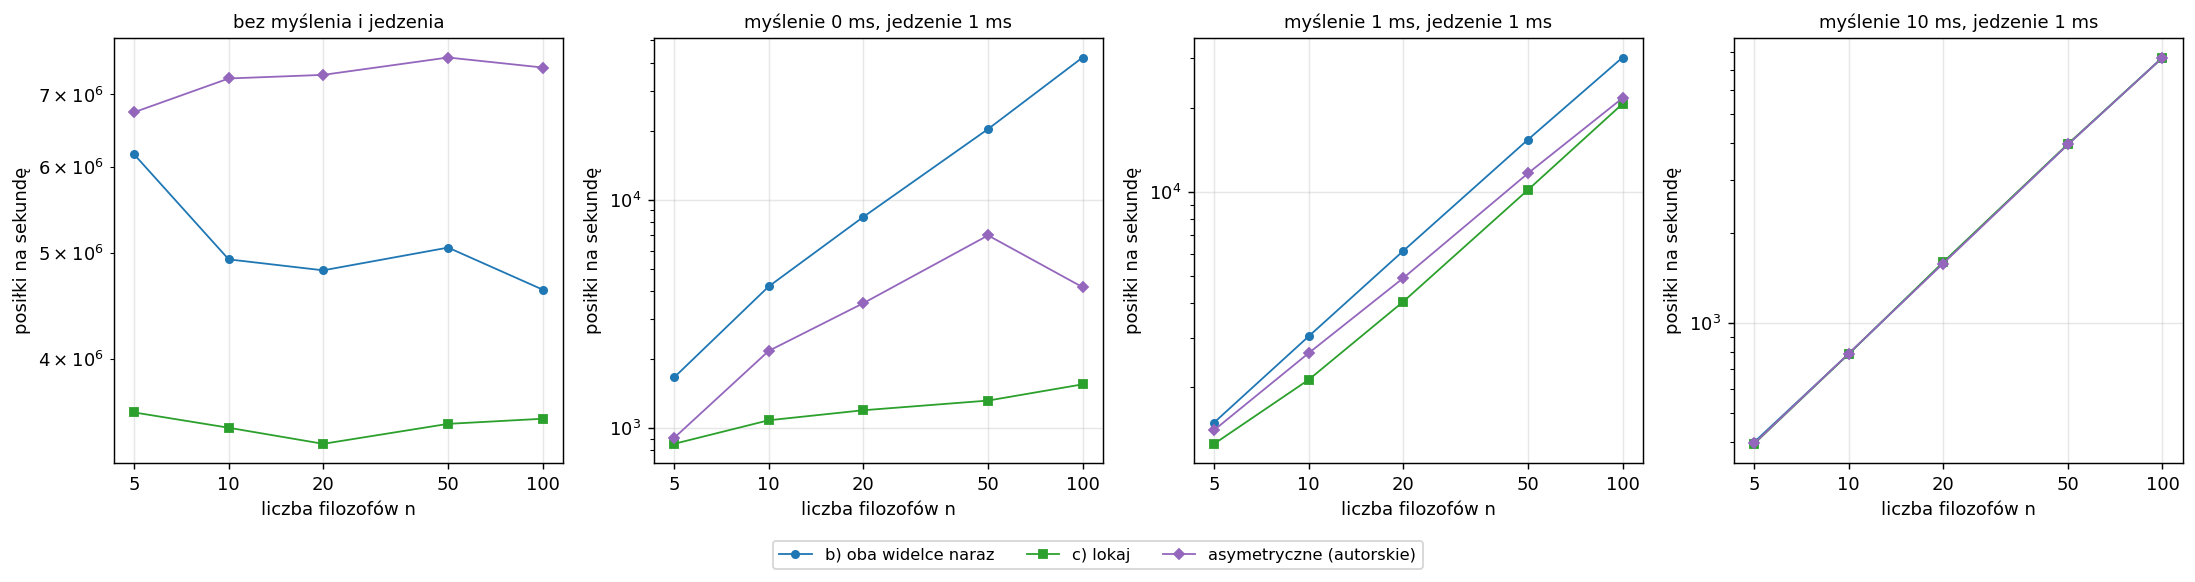
\includegraphics[width=\textwidth]{img/throughput.png}
    \caption{Przepustowość w zależności od liczby filozofów}
\end{figure}

\textbf{Tabela 1} zestawia mediany dla $n = 5$ i $n = 100$.

\begin{table}[H]
    \centering
    \renewcommand{\arraystretch}{1.3}
    \begin{tabular}{|l|l|r|r|r|r|r|r|}
        \hline
        \multirow{2}{*}{\textbf{Scenariusz}} & \multirow{2}{*}{\textbf{Rozwiązanie}} & \multicolumn{3}{c|}{$n = 5$} & \multicolumn{3}{c|}{$n = 100$} \\ \cline{3-8}
        & & posiłki/s & czekanie [\textmu s] & $J$ & posiłki/s & czekanie [\textmu s] & $J$ \\ \hline
        \multirow{3}{*}{0/0} & b) oba naraz & \num{6163329} & \num{0.6} & \num{1.00} & \num{4630063} & \num{16.1} & \num{0.98} \\
         & c) lokaj & \num{3569841} & \num{1.1} & \num{1.00} & \num{3522370} & \num{15.0} & \num{0.99} \\
         & asymetryczne & \num{6740508} & \num{0.6} & \num{0.48} & \num{7409489} & \num{13.4} & \num{0.02} \\ \hline
        \multirow{3}{*}{0/1} & b) oba naraz & \num{1668} & \num{1803.4} & \num{0.77} & \num{42099} & \num{1213.0} & \num{0.50} \\
         & c) lokaj & \num{853} & \num{4611.2} & \num{0.32} & \num{1555} & \num{67170.1} & \num{0.04} \\
         & asymetryczne & \num{906} & \num{4264.8} & \num{0.34} & \num{4147} & \num{24532.0} & \num{0.14} \\ \hline
        \multirow{3}{*}{1/1} & b) oba naraz & \num{1499} & \num{941.5} & \num{1.00} & \num{30188} & \num{985.4} & \num{1.00} \\
         & c) lokaj & \num{1258} & \num{1578.8} & \num{1.00} & \num{20619} & \num{2528.9} & \num{1.00} \\
         & asymetryczne & \num{1409} & \num{1185.9} & \num{0.99} & \num{21616} & \num{2311.9} & \num{0.99} \\ \hline
        \multirow{3}{*}{10/1} & b) oba naraz & \num{400} & \num{194.0} & \num{1.00} & \num{7695} & \num{145.9} & \num{1.00} \\
         & c) lokaj & \num{395} & \num{221.7} & \num{1.00} & \num{7688} & \num{168.3} & \num{1.00} \\
         & asymetryczne & \num{396} & \num{194.4} & \num{1.00} & \num{7688} & \num{160.8} & \num{1.00} \\ \hline
    \end{tabular}
    \caption{Przepustowość, średni czas oczekiwania na widelce i indeks Jaina $J$}
\end{table}

Bez myślenia i jedzenia (0/0) najszybsze jest rozwiązanie asymetryczne: 6,7--7,4 mln posiłków na
sekundę, bo każdy widelec synchronizuje tylko dwóch sąsiadów i nie ma wspólnego monitora.
Rozwiązanie b) jest wolniejsze (4,6--6,2 mln), a dla $n \ge 10$ wyraźnie traci, bo każdy posiłek
przechodzi przez jeden monitor stołu, a \texttt{notifyAll()} budzi wszystkich czekających.
Lokaj jest najwolniejszy (3,5 mln) -- każdy posiłek to dwa wejścia do wspólnego monitora lokaja
i cztery do monitorów widelców.

Przy jedzeniu 1 ms koszt synchronizacji jest pomijalny, a przepustowość zależy od tego,
ilu filozofów je jednocześnie. W scenariuszu 10/1 filozofowie rzadko konkurują,
wszystkie rozwiązania osiągają ten sam wynik, rosnący liniowo z $n$ (nieco poniżej
$\frac{n}{11\,\text{ms}}$ ze względu na narzut \texttt{parkNanos}).
W scenariuszu 1/1 najlepsze jest rozwiązanie b), bo filozof nie zajmuje widelca, z którego nie może
skorzystać. W pozostałych rozwiązaniach filozof trzymający jeden widelec blokuje sąsiada,
mimo że sam jeszcze nie je, i powstają łańcuchy oczekujących filozofów.

Największe różnice są w scenariuszu 0/1 (ciągle głodni filozofowie). Rozwiązanie b) osiąga
dla $n = 100$ 42 tys. posiłków na sekundę, czyli blisko maksimum $\frac{n}{2}$ jedzących naraz
($50$ tys.). Rozwiązanie asymetryczne osiąga 4,1 tys., a lokaj tylko 1,6 tys. posiłków na sekundę --
mniej niż 2 filozofów je jednocześnie. Filozof, który odłożył widelce, natychmiast próbuje
podnieść je ponownie, więc niemal każdy widelec jest zajęty przez kogoś, kto czeka na drugi,
i tworzą się długie łańcuchy oczekiwania. Przy lokaju dodatkowo kolejność wpuszczania do stołu
nie ma związku z dostępnymi widelcami.

\subsection{Czas oczekiwania}
\textbf{Rysunki 4 i 5} pokazują średni i maksymalny czas oczekiwania na widelce.

\begin{figure}[H]
    \centering
    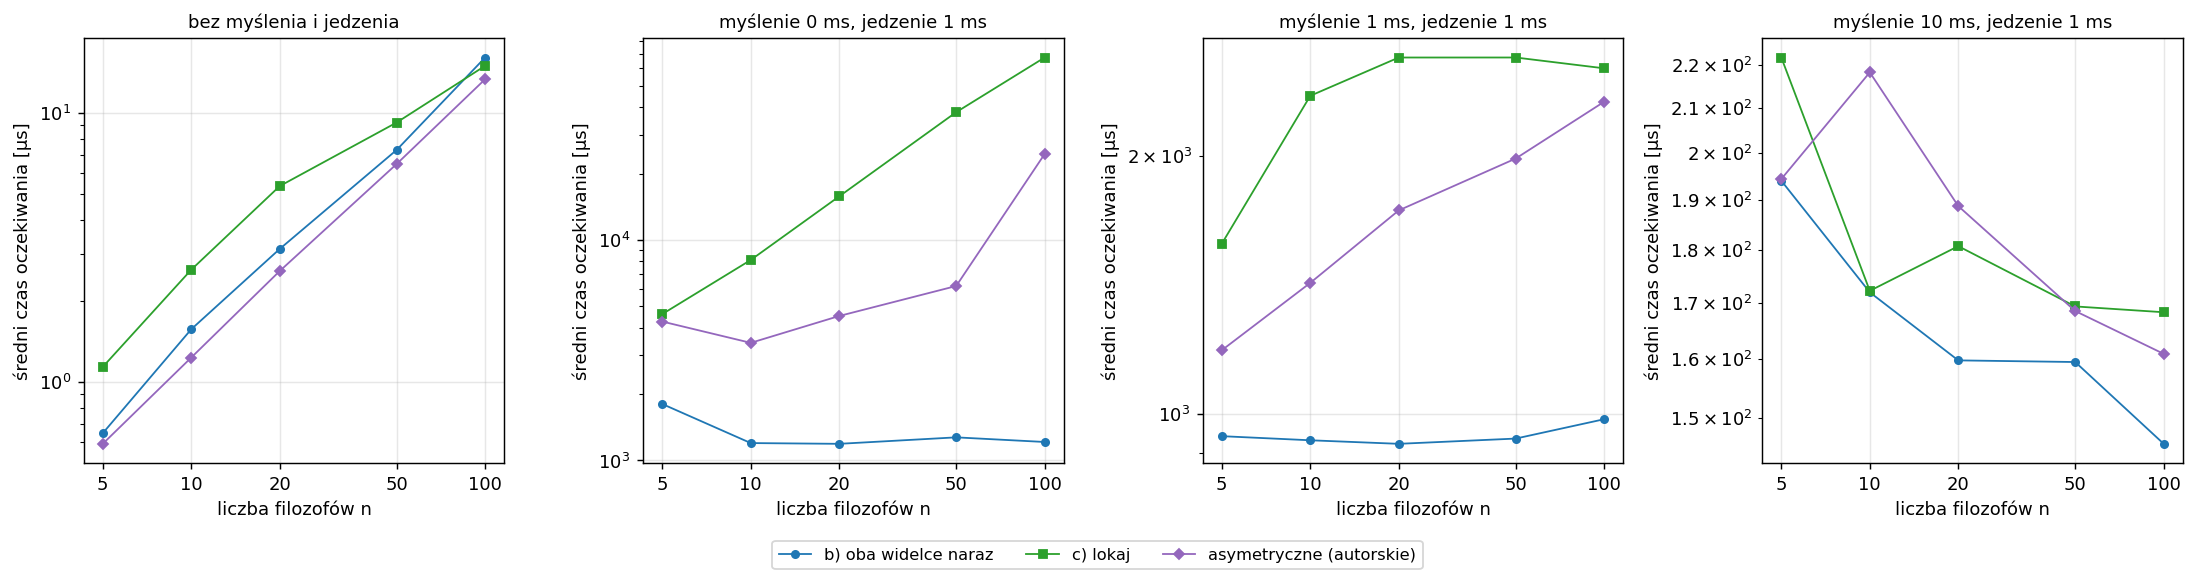
\includegraphics[width=\textwidth]{img/wait_mean.png}
    \caption{Średni czas oczekiwania na widelce}
\end{figure}

\begin{figure}[H]
    \centering
    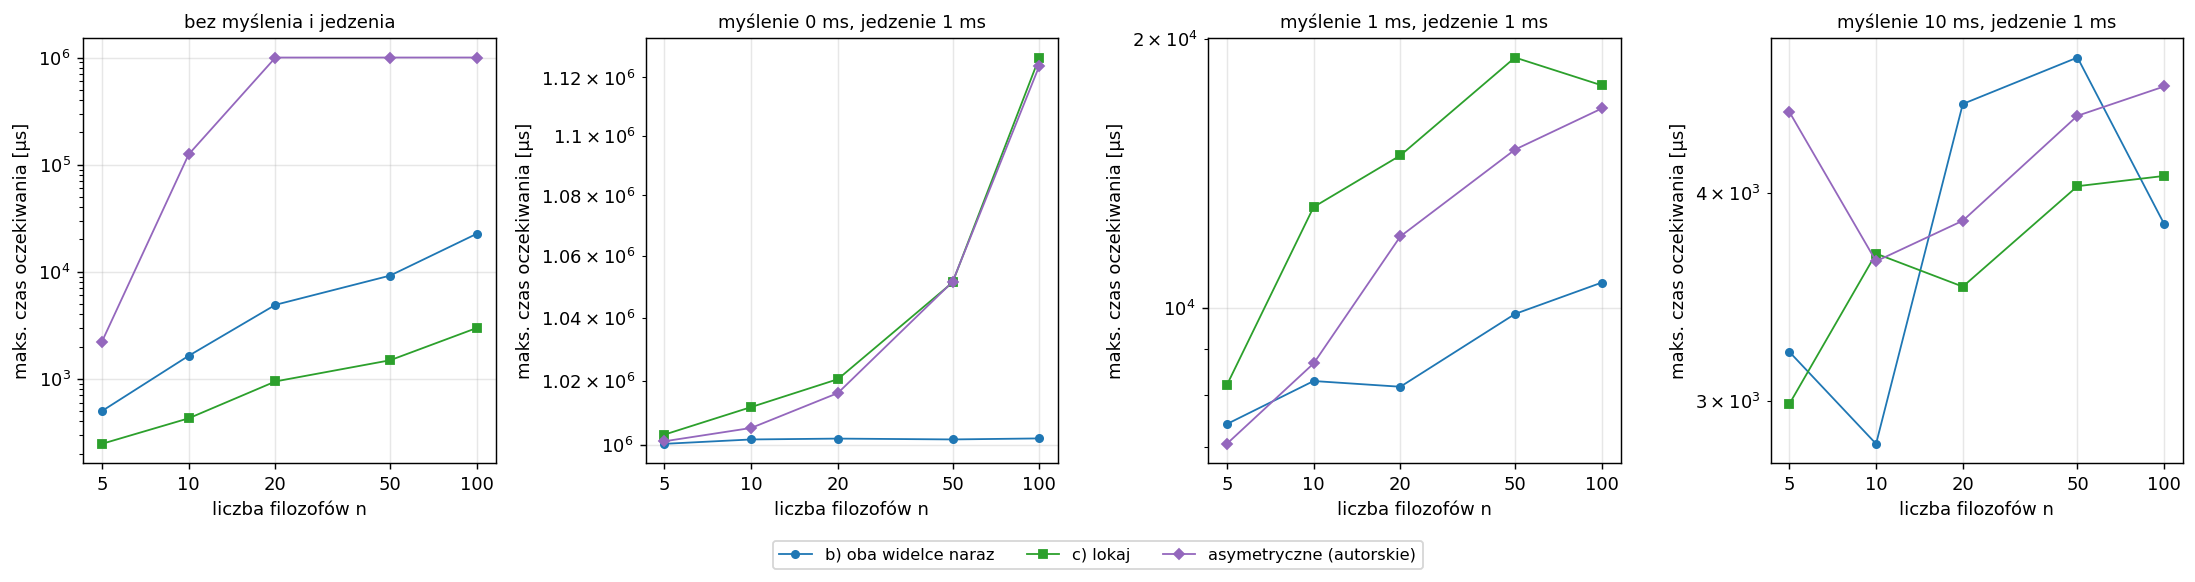
\includegraphics[width=\textwidth]{img/wait_max.png}
    \caption{Maksymalny czas oczekiwania na widelce}
\end{figure}

Średnie czasy odpowiadają przepustowości: przy małej rywalizacji (10/1) filozof czeka
średnio 150--220 \textmu s, a w scenariuszu 0/1 dla $n = 100$ od 1,2 ms (b) do 67 ms (lokaj).
Maksymalny czas oczekiwania w scenariuszu 0/1 dla wszystkich rozwiązań wynosi około 1 s,
czyli cały przebieg: niektórzy filozofowie doczekali się widelców dopiero wtedy, gdy
pozostali kończyli pracę. Bez myślenia i jedzenia to samo dotyczy rozwiązania asymetrycznego
dla $n = 100$.

\subsection{Sprawiedliwość}
\textbf{Rysunek 6} pokazuje indeks Jaina liczby posiłków. Przerywana linia $\frac{1}{n}$
odpowiada sytuacji, w której je tylko jeden filozof.

\begin{figure}[H]
    \centering
    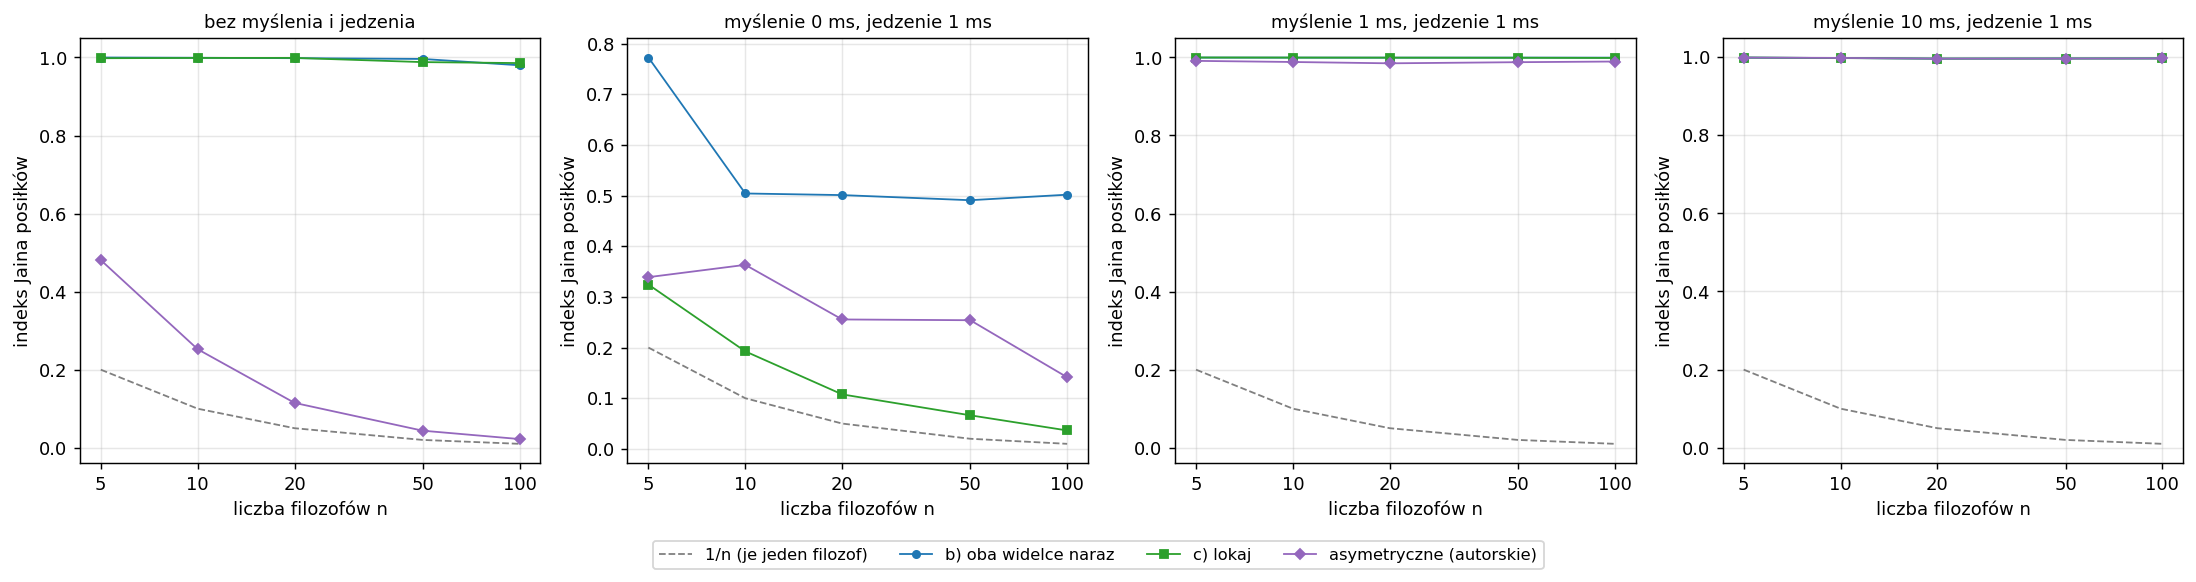
\includegraphics[width=\textwidth]{img/jain.png}
    \caption{Indeks Jaina liczby posiłków}
\end{figure}

Gdy filozofowie myślą (1/1 i 10/1), wszystkie rozwiązania są sprawiedliwe ($J \ge 0{,}99$).
Gdy nie myślą (0/1), wszystkie głodzą filozofów. W rozwiązaniu b) dla $n \ge 10$ $J \approx 0{,}5$:
je co drugi filozof, a jego sąsiedzi prawie wcale. W rozwiązaniu z lokajem i asymetrycznym $J$ spada dla $n = 100$
do 0,04 i 0,14, czyli blisko $\frac{1}{n}$. Bez myślenia i jedzenia (0/0) b) i lokaj są sprawiedliwe,
a rozwiązanie asymetryczne nie (dla $n = 100$ $J = 0{,}02$).

Przyczyna jest ta sama co w laboratorium 4: monitor Javy nie gwarantuje kolejności wejścia.
Filozof, który odłożył widelec (\textsc{notify}), od razu wywołuje \textsc{take} ponownie i zwykle
zdobywa monitor widelca, zanim obudzony sąsiad zdąży się wykonać. Przerwa na myślenie daje
sąsiadowi czas na zabranie widelca, dlatego w scenariuszach 1/1 i 10/1 problem znika.

\subsection{Zagłodzenie przez sąsiadów}
\textbf{Rysunek 7} pokazuje wynik eksperymentu z dwoma żarłocznymi filozofami F1 i F3.

\begin{figure}[H]
    \centering
    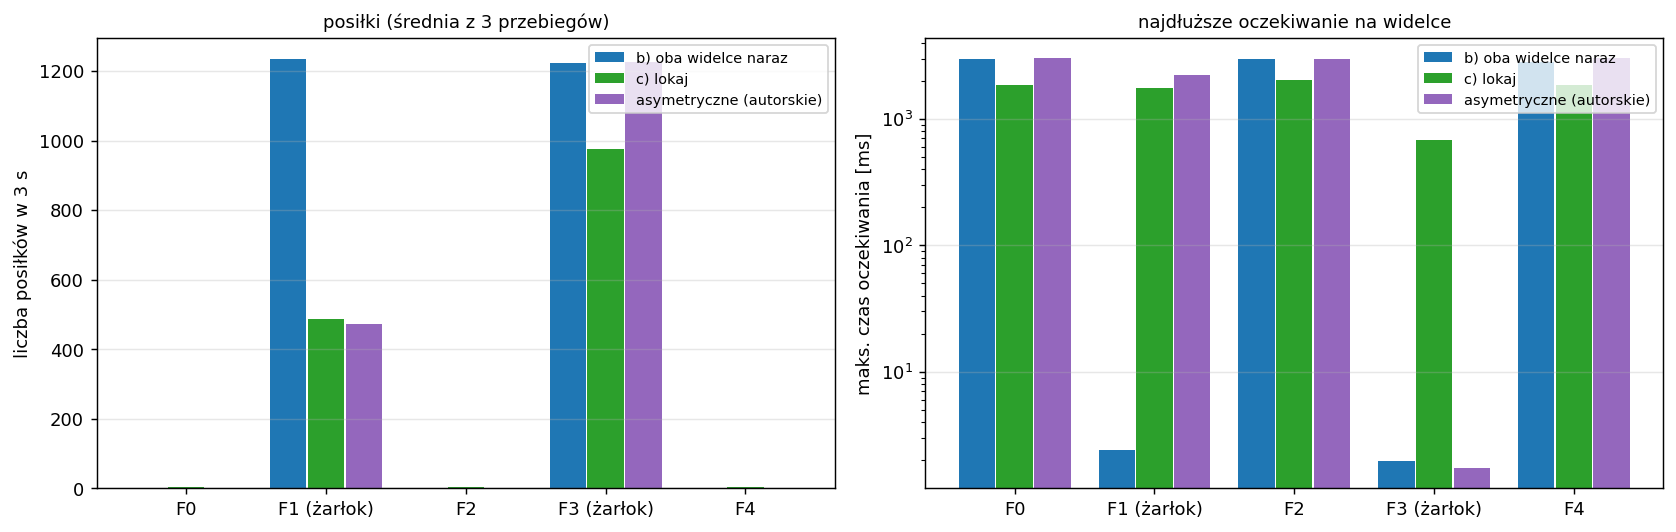
\includegraphics[width=\textwidth]{img/starvation.png}
    \caption{Liczba posiłków i najdłuższe oczekiwanie, F1 i F3 nie myślą, $n = 5$, 3 s}
\end{figure}

W rozwiązaniu b) żarłoki zjadły średnio 1233 i 1224 razy, a F0, F2 i F4 tylko 2, 1 i 2 razy
w ciągu 3 s. Najdłuższe oczekiwanie F2 wyniosło 3{,}00 s, czyli praktycznie cały przebieg.
To dokładnie scenariusz zagłodzenia z rozdziału 3.2: F1 i F3 nie są sąsiadami, więc mogą jeść
jednocześnie i na zmianę, a F2 potrzebuje chwili, w której nie je żaden z nich.
W rozwiązaniu z lokajem i asymetrycznym F0, F2 i F4 również jedzą tylko kilka razy,
ale żarłoki też tracą (472--976 posiłków), bo czekają na widelce trzymane przez sąsiadów,
którzy czekają na drugi widelec. Żadne z badanych rozwiązań nie chroni przed zagłodzeniem,
gdy niektórzy filozofowie nie dają innym szansy.

\section{Wnioski}
Rozwiązanie trywialne prowadzi do blokady. Przy dużej rywalizacji następuje ona w ułamku
milisekundy, a przy długim myśleniu może nie wystąpić przez długi czas, co czyni błąd trudnym
do wykrycia w testach.

Rozwiązanie z widelcami podnoszonymi jednocześnie nie może się zablokować, ale może zagłodzić
filozofa, którego sąsiedzi jedzą na zmianę. Gdy jedzenie trwa dłużej niż synchronizacja,
jest najwydajniejsze ze wszystkich, bo nikt nie trzyma widelca bez jedzenia. Jego słabością jest
jeden monitor stołu i \texttt{notifyAll()}, co widać, gdy jedzenie jest krótkie, a filozofów dużo.

Lokaj usuwa blokadę najmniejszą zmianą rozwiązania trywialnego, ale jest najwolniejszy:
wspólny monitor jest wąskim gardłem, a przy dużej rywalizacji ograniczenie do $n - 1$ filozofów
nie zapobiega długim łańcuchom oczekiwania na widelce.

Rozwiązanie asymetryczne nie ma wspólnego punktu synchronizacji i ma najmniejszy koszt
synchronizacji, ale przy dużej rywalizacji jest niesprawiedliwe.

Na wydajność wpływają więc przede wszystkim: stopień rywalizacji (stosunek czasu myślenia do jedzenia),
to, czy filozof może trzymać widelec bez jedzenia, obecność wspólnego monitora
(stół w b), lokaj w c)) oraz liczba niepotrzebnie budzonych wątków. Gwarancji braku zagłodzenia
nie daje żadne z rozwiązań opartych na monitorach Javy, bo nie zachowują one kolejności oczekujących.
Uzyskanie jej wymagałoby kolejki FIFO lub priorytetu dla najdłużej głodnego filozofa,
kosztem przepustowości, podobnie jak kolejka biletowa w laboratorium 4.

\begin{thebibliography}{9}
    \bibitem{dijkstra} E.W. Dijkstra: \textit{Hierarchical ordering of sequential processes}. Acta Informatica 1(2), 1971.
    \bibitem{coffman} E.G. Coffman, M. Elphick, A. Shoshani: \textit{System Deadlocks}. ACM Computing Surveys 3(2), 1971.
    \bibitem{agh} \url{https://home.agh.edu.pl/~funika/tw/lab5/}
    \bibitem{java} \url{https://docs.oracle.com/javase/specs/jls/se27/html/jls-17.html}
\end{thebibliography}

\end{document}
